\section{Discussion}
\label{section:p450/discussion}
The physical score performs nearly as well as the fitted score indicating that the model is not overfit to the training set.
Figure \ref{figure:idsite_other} presents a comparison of both IDSite models (physical and fit) to a number of other methods for prediction of P450 sites of metabolism.
Though the data sets used are not identical they are similar and overlapping for some compounds.
At all sensitivities IDSite is clearly the best performing protocol, with the physical and fit model performing very nearly identically.

At 90\% sensitivity, the QSAR method included roughly 20\% false positives, and MetaSite included 40\% false positives.
At the same sensitivity IDSite has a \textapprox1\% false positives rate.
This represents a significant improvement in prediction accuracy that has the potential to have a large impact on drug development.

\subsection{Significance of Sampling Stages}
\label{subsection:p450/discussion/sampling_stages}
\begin{figure}[h!]
\centering
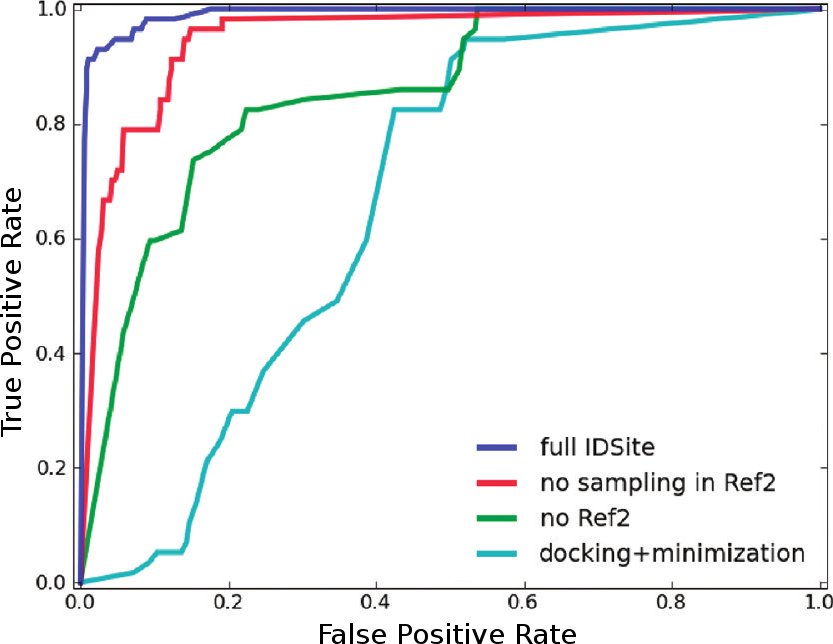
\includegraphics[width=0.5\textwidth]{figures/idsite/roc_sampling.png}
\caption{The effect of additional sampling on prediction of site of metabolism by P450.
The light blue series describes only performing the initial Glide docking stage followed by minimization.
The green series is obtained by using the set of structures obtained in the first minimization Monte Carlo sampling stage.
The red series is obtained by screening the structures obtained in the first sampling stage, and minimizing these structures using the constraints specified in Figures \ref{figure:second_sp2_constraints} and \ref{figure:second_sp3_constraints}.
The blue series makes use of the entire IDSite procedure.
The color scheme of these series corresponds to the colors of edges in Figure \ref{figure:idsite_overview}.}
\label{figure:idsite_roc_sampling}
\end{figure}

As shown in Figure \ref{figure:idsite_roc_sampling} at a given specificity, sensitivity increases with additional sampling.
For some compounds there are either no conformations predicted via the docking procedure where the site of metabolism is sufficiently close to the heme oxygen to react or the scoring metric used by the docking procedure prefers conformations which are far from the reactive site over more reactive conformations.
The sampling stages, and constraints are useful in guiding these initial docked poses into more active conformations.

The trajectory followed duing the minimization Monte Carlo sampling stages differs appreciably for small and large ligands.
For smaller ligands, in many cases the poses after the first constrained minimization were among the lowest energy poses explored.
For about 40\% of these small ligands (24/56) the same predictions were obtained after the first minimization Monte Carlo sampling stage as after the full IDSite procedure.
However, for large ligands, the constraings and sampling continued to decrease the energy over the course of the sampling stages, indicating that especially for large compounds the second refinement stage is critical to obtaining accurate predictions.

\subsection{Induced Fit Effects}
\label{subsection:p450/discussion/induced_fit}



\subsection{Significance of Structure in Predicting Sites of Metabolism}
\label{subsection:p450/discussion/structure_effects}
